%================================================================================================
%================================= PRIMEIRA FOLHA INTERNA  ======================================
%================================================================================================
\begin{figure}
\center

\includegraphics[height=0.15\textwidth]{Figs/logoCefetCampusPetropolis.jpg} 
\end{figure}


\vspace*{0.8cm}

\begin{center}
{\large \bf CENTRO FEDERAL DE EDUCAÇÃO TECNOLÓGICA} \vspace{1mm} \\
{\large \bf CELSO SUCKOW DA FONSECA - CEFET/RJ \textit{CAMPUS} PETRÓPOLIS} \vspace{1mm} \\
{\large \bf CURSO: BACHARELADO EM ENGENHARIA DE COMPUTAÇÃO}\\

\vspace*{5cm}
{\large \bf PREVISÃO NEURAL DE TENDÊNCIAS DE VALORES FUTUROS DO BITCOIN}\\
\end{center}
\vspace{4cm}
\hfill
%\begin{minipage}%{0.45\linewidth}
	\begin{flushright}
	Bernardo Botelho Antunes da Costa
	\end{flushright}
%\end{minipage}


\vspace*{3.3cm}
\begin{center}
{\bf PETRÓPOLIS \\ 2018}\\
\end{center}

%--------------------------------------------------------------------------
%--------------------------------------------------------------------------
\newpage
\pagestyle{empty}

\begin{center}
{\large \bf CENTRO FEDERAL DE EDUCAÇÃO TECNOLÓGICA} \vspace{1mm} \\
{\large \bf CELSO SUCKOW DA FONSECA - CEFET/RJ \textit{CAMPUS} PETRÓPOLIS} \vspace{1mm} \\
{\large \bf CURSO: BACHARELADO EM ENGENHARIA DE COMPUTAÇÃO}

\vspace*{3cm}
\normalsize{\large \bf PREVISÃO NEURAL DE TENDÊNCIAS DE VALORES FUTUROS DO BITCOIN}\\
\end{center}
\vspace{1.5cm}
\hfill
%\begin{minipage}%{0.45\linewidth}
	\begin{flushright}
	Bernardo Botelho Antunes da Costa
	\end{flushright}
%\end{minipage}
\vspace*{1.5cm}
\begin{flushright}
	\begin{minipage}{0.5\textwidth}
		{\normalsize
		Trabalho de Conclusão de Curso apresentado ao  
	 CEFET/RJ -{\it campus} Petrópolis, como parte dos requisitos para obtenção do título de Bacharel em Engenharia de Computação.}
	\end{minipage}\\[1.5cm]
\end{flushright}
\vspace{1.5cm}
\hfill
%\begin{minipage}%{0.45\linewidth}
\begin{flushright}
Orientador: Prof. Diego Barreto Haddad, D.Sc.
\end{flushright}




\vspace*{3.3cm}
\begin{center}
{\bf PETRÓPOLIS \\ 2018}\\
\end{center}



%--------------------------------------------------------------------------
%--------------------------------------------------------------------------
\newpage
\begin{minipage}{0.9\textwidth}

{\normalsize 
\begin{center}
Autorizo(amos) a reprodução e divulgação total ou parcial deste trabalho, por qualquer meio
eletrônico ou convencional, para fins de estudo e pesquisa, desde que citada a fonte.
\end{center}
\vspace*{0.5cm}
}
\end{minipage}
\vspace*{5cm}
\begin{center}
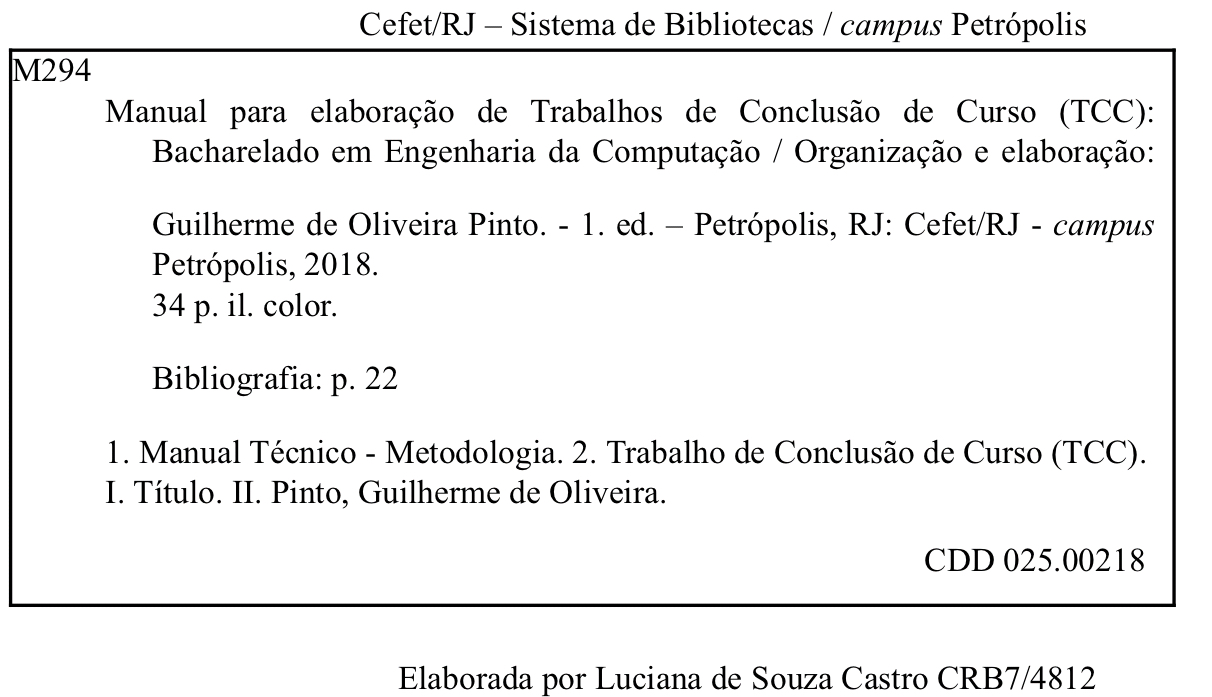
\includegraphics[height=0.4\textwidth]{Figs/biblioteca_engcomp.jpeg} 
\end{center}






%--------------------------------------------------------------------------
%--------------------------------------------------------------------------

\newpage
\newcommand{\HRule}{\rule{0.6\linewidth}{0.5mm}}
\pagestyle{empty}

{\center % Center everything on the page


\begin{figure}
\center

\includegraphics[height=0.13\textwidth]{Figs/logoCefetCampusPetropolis.jpg} 
\end{figure}

\begin{center}
{\large \bf CENTRO FEDERAL DE EDUCAÇÃO TECNOLÓGICA} \vspace{1mm} \\
{\large \bf CELSO SUCKOW DA FONSECA - CEFET/RJ \textit{CAMPUS} PETRÓPOLIS} \vspace{1mm} \\
{\large \bf CURSO: BACHARELADO EM ENGENHARIA DE COMPUTAÇÃO}\\
\vspace*{1.2cm}
{\large  FOLHA DE APROVAÇÃO}

\vspace*{1.3cm}
{\large \bf  Previsão Neural de Tendência de Valores Futuros do Bitcoin}\\
\end{center}
\vspace{0.5cm}
\hfill
%\begin{minipage}%{0.45\linewidth}
\begin{flushright}
    Bernardo Botelho Antunes da Costa
	\end{flushright}
%\end{minipage}
\vspace*{0.5cm}
\begin{flushright}
	\begin{minipage}{0.5\textwidth}
		{\normalsize
		Trabalho de Conclusão de Curso apresentado ao  
	 CEFET/RJ -{ {\it campus} Petrópolis}, como parte dos requisitos para obtenção do título de Bacharel em Engenharia de Computação.}
	\end{minipage}\\[0.5cm]
\end{flushright}
\vspace{0.5cm}
\hfill
%\begin{minipage}%{0.45\linewidth}
\begin{flushright}
Orientador: Prof. Diego Barreto Haddad
\end{flushright}

\begin{minipage}{0.9\textwidth}
	\begin{flushleft}
	Aprovado por:
	\end{flushleft}
\end{minipage}\\[1cm]

\center
\HRule \\
Prof. Diego Barreto Haddad, D.Sc. (Orientador) \\[0.4cm]
\HRule \\
Prof. Luís Domingues Tomé Jardim Tarrataca, D.Sc.\\[0.4cm]
\HRule \\
Profa. Laura Silva de Assis, D.Sc.  \\[1.5cm]


\begin{center}
{Agosto de 2018}
\end{center}


}



\newpage


% Dedicat�ria
%\begin{center}
%\textbf{\large DEDICATÓRIA}
%\end{center}
%      \vspace{0.5cm}
%
%Opcional.
%\newpage



% Agradecimento
\begin{center}
\textbf{\large  AGRADECIMENTO}
\end{center}
      \vspace{0.5cm}

Dedico este trabalho ao povo brasileiro que contribuiu de forma significativa a minha formação e estada nesta Universidade. Este projeto é uma pequena forma de retribuir o investimento a mim depositados, de forma compulsória, com a exígua esperança de fomentar o desenvolvimento econômico e tecnológico da nação.



\newpage


% Resumo
\begin{center}
\textbf{\large RESUMO}
\end{center}
      \vspace{0.5cm}
      
 Este trabalho apresenta uma estudo de previsão da série temporal do Bitcoin usando Redes Neurais, utilizando para isso, os dados do valor do preço do Bitcoin e os valores de tendência de pesquisa, que são encontrados no \textit{Google Trends}. Para isso foram utilizados os algoritmos do PCA para redução da dimensão da base de dados, reduzindo a necessidade de poder de processamento; O \textit{Backpropagation} para o calculo dos pesos da Rede; O \textit{K-fold} para escolha da arquitetura da rede a ser usada no modelo. Com o objetivo de reduzir a variância e aumentar a acurácia do sistema, também foi foi utilizada a técnica do \textit{ensemble}.

 Para comparar os resultados obtidos com os resultados apresentados  em trabalhos anteriores, foram utilizados dados no do dia 19 de Agosto de 2013 até 19 de Julho de 2016. 
 
 Como resultado, a abordagem deste trabalho obteve acurácia 53,99\%, utilizando os dados do valor do preço do Bitcoin e o valor do \textit{Google Trends} do termo Bitcoin, enquanto o máximo obtido em trabalhos anteriores foi de 52,78\%, utilizando apenas os dados do valor do preço do Bitcoin, o que significa um aumento de 1,21\%.
 
 Entretanto, o acurácia ainda está muito abaixo de uma valor no qual seria possível obter lucros superiores ao mercado. Tal dificuldade pode ser explicada pela teoria de mercado eficiente, que diz que não seria possível obter lucros acima da média do mercado sem levar em conta a sorte ou o uso de informações privilegiadas.


\begin{flushleft}
{\bf Palavras-chaves:} Previsão, Bitcoin, \textit{Google Trends}, Redes neurais.
\end{flushleft}

\newpage

\begin{center}
\textbf{\large ABSTRACT}
\end{center}
\vspace{0.5cm}

This work presents a prediction study of the Bitcoin time series using Neural Networks, utilizing Bitcoin price values and the trend values of web search, which are enables in Google Trends. For this, we use the  PCA algorithms to reduce the size of the dataset, reducing the demand for processing. We use Backpropagation to compute the network weight. In order to select the best network architecture, we use the K-fold algorithm.  Finally, we use the ensemble technique to reduce variance and increase the accuracy of the system.

 With the objective to compare the results that we obtain with the previous studies results, we use the dataset from August 19, 2013, until July 19, 2016.
 
 As the result of this study, our approach presented by this paper got an accuracy of 53.99\%, applying dataset from Bitcoin's price and  Bitcoin's Google Trends, while the maximum achieved in previous works was 52.78\%, using only Bitcoin's price dataset, which means that we increase the accuracy to 1.21\%.
 
 However, the accuracy is still no good enough to obtain greater profits than to the market. We attribute this difficulty to the efficient market theory whereby should be impossible to outperform the overall market, unless though luck or some insider information.


\begin{flushleft}
{\bf Key-words:} Forecasting, Bitcoin,\textit{Google Trends}, Neural Networks.
\end{flushleft}
